\chapter{EVENT RECOGNITION}
 \label{chap:eventrec}
 \section{Introduction}
Visual event recognition has been observed as a potential area of research in several applications like  content-based video retrieval, human computer interaction and more. 
In general the visual event recognition are always modelled as stochastic temporal processes in the semantic space. The motivation behind it is to capture the dynamic patterns of event through collective evolution of the semantic concept. One of the most familiar method following this approach is Hidden Markov Model (HMM) which has been a favourite for the sequential pattern recognition. However, the HMM's have struggled to incorporate both spatial and temporal context present in the event.  
\par In another approach by ~\cite{YanKe05}, event is treated as a space-time volume in the video sequence. Volumetric features based on optical flow are extracted for event detection. These are generally used for videos having only single moving object (human) and action. For complex activity recognition \citep{YanKe07}, the internet videos are already temporarily localized and they focus on identifying the primitive event.
\par A common approach for video classification ~\citep{Liu09}~\citep{Niebles10} involves : extracting local region level features, combining features to fixed size video level description and trained a classifier on the features to predict the class labels. But in these approaches feature extraction plays a crucial role, and features must be revisited again for different videos. Convolutional Neural Network(CNN) replace all three stages with a single neural network ~\cite{Ji13}, it is trained end to end from raw pixel values to classifier outputs. However CNN was observed to be computationally expensive and took longer training period to effectively optimize. With the improvements on GPU hardware,CNN's could be scaled to train networks of millions of parameters.

\par Section \ref{sec:cnn} outlines the overall framework of CNN and would discuss the reason for choosing it for event recognition task over the existing techniques. Then we will elaborate the architecture and features supported by the indigenous deep neural network tool kit designed in python in Section \ref{sec:pyDNN}. 

\section{Convolutional Neural Network (CNN)}
 \label{sec:cnn}
 \par Covolutional neural networks (CNN) are variant of multi-layer perceptron (MLP) that are designed by studying the complex arrangement of cells in the cats visual cortex. It comprise of one or more convolutional layers (often with a sub-sampling step), followed by one or more standard MLP. There are different varieties of CNN based on the dimensionality of input and convolution operator, like CNN-2D, CNN-3D etc. A major advantage of having CNN is that it learns faster (fewer parameters) compared to  MLP with the same number of hidden units. CNN  also use  gradient based optimization to compute parameters of the model. It is  evident that CNN fits very well onto the visual recognition domain, as it handles very high dimensional data, exploits the topology of image or video and is invariant to small translation and illumination changes.  CNN leverage following concepts to tackle the above mentioned challenges,
\subsection{Local Connectivity}
It exploits the spatially local correlation , allowing only local connectivity between neurons of adjacent layers. Hence, every hidden units is only sensitive to a small block in the visual field, called receptive field. This drastically reduce the number of connections between input and hidden layer which therefore diminishes the number of parameters needed to train the model.
\subsection{Shared Filters}
The hidden units are associated to the receptive field by filters which are shared within a feature map. These filters captures edge like patterns within the receptive field. Additionally, sharing filters increases learning efficiency by greatly reducing the number of free parameters to be learned. Apart from reducing parameters, they extract the same feature at every position, which makes every feature map to be equi-variant to any changes in the input. The shared filters are associated to the receptive field by a dot product operation which can be expressed as a discrete convolution operation.
\subsection{Pooling/Sub-sampling Hidden Units}
The sub-sampling layer pools the hidden unit output in the non-overlapping neighbourhood. Pooling can be either average or maximum.  The max pooling provides local translation in-variance and is commonly being used. Pooling also reduces inputs to next layer of feature extraction. With pooling the feature maps in latter layer extracts coarser features.

\par All these concepts empower CNN to achieve better generalization in the vision problems. Stacking multiple such layers is very common approach to attain better responsiveness over a larger visual field. Some architectural tricks such as rectification and contrast normalization are tried for improved result on a large dataset. The unsupervised pre-training of each filter weight, has helped enhance the robustness of the models built.

\section{Python-DNN Toolkit}
\label{sec:pyDNN}
Neural networks can be best implemented using modular, object-oriented approach. Where each models (dnn, sda, cnn) are implemented as a different class with member functions performing pre-training (an unsupervised learning), fine-tuning (supervised learning), testing , loading and saving the model. This approach enable reuse of the code for the most of the network models. Even though the most of existing toolkits were sophisticated, these toolkits were hard to configure, configuration were either through command line or arguments to a function. Since neural networks take too many parameters, it gets difficult to understand the purpose of a parameter Hence  \textit{Python-DNN} toolkit was developed.  
\subsection{Architecture}
The tollkit was implemented in python using the numerical computation library named  \textit{Theano}. It provides platform to run efficiently in CPU and GPU architecture.
Architecture of the indigenous DNN toolkit is shown on \ref{fig:architecture}.
\begin{figure}[htpb]
   \begin{center}
	    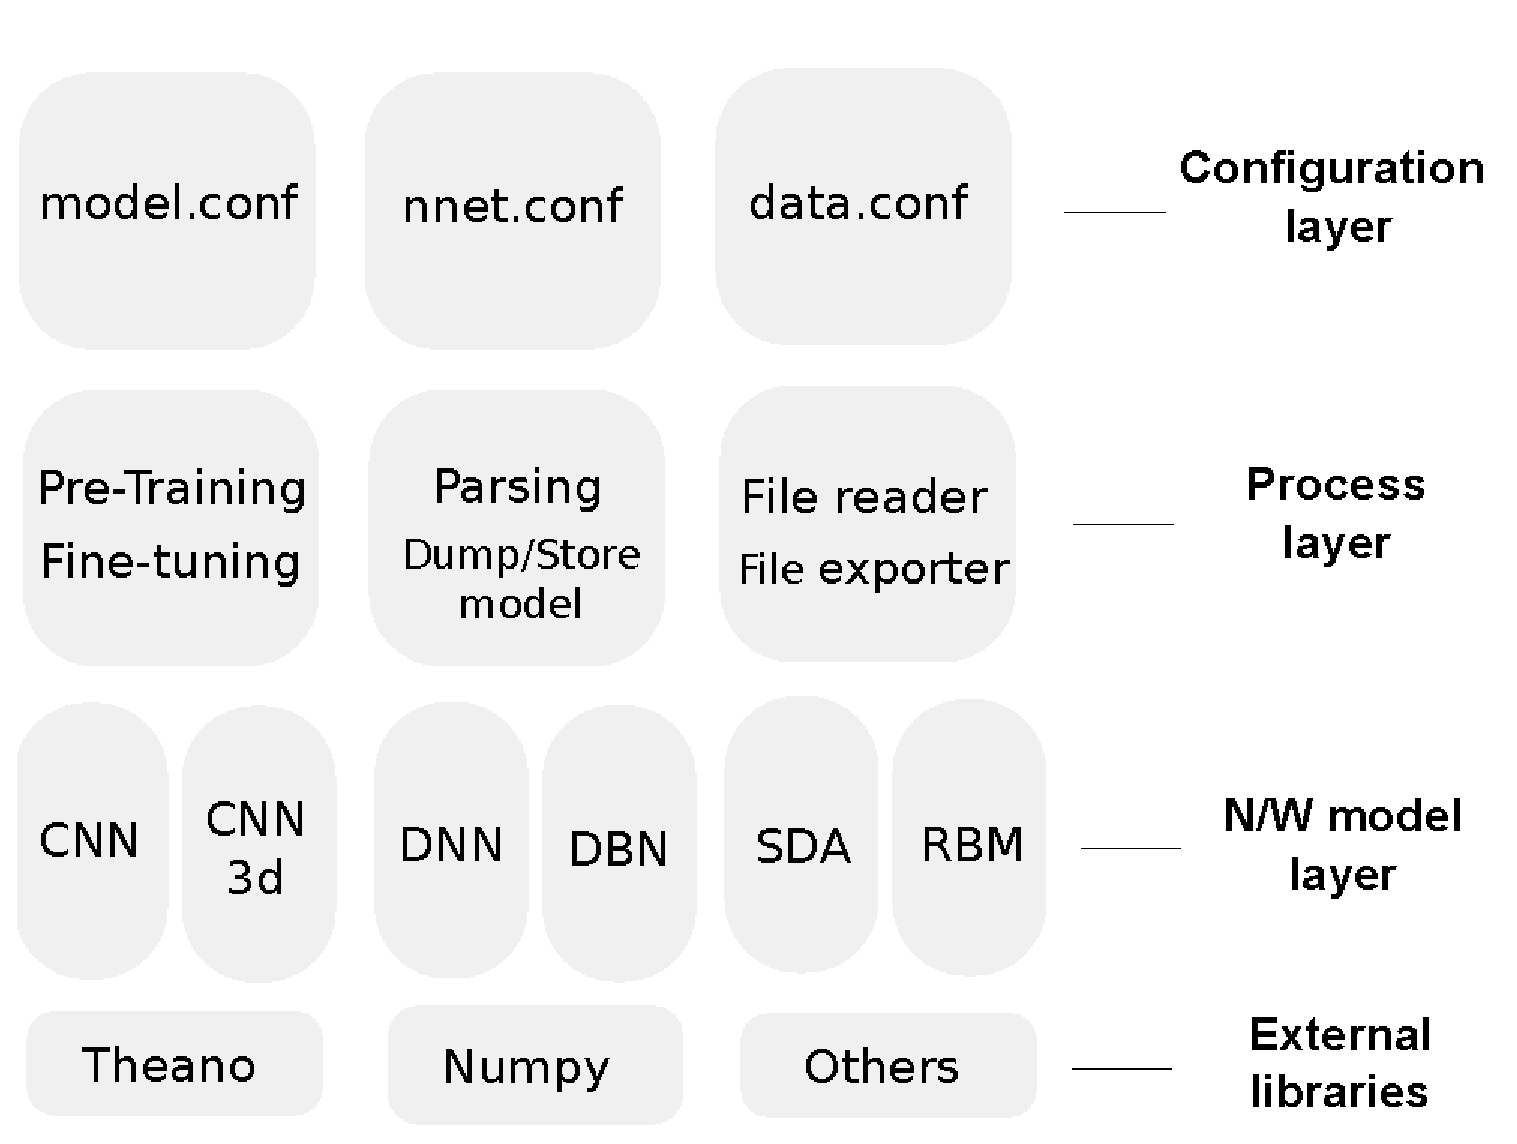
\includegraphics[width=0.75\textwidth]{snaps/architecture.eps}     
     \caption {Python-DNN Architecture}
	 \label{fig:architecture}
   \end{center}
 \end{figure}
 Toolkit has been split into four layers : external libraries that includes all the dependent libraries, network model layer that encompass different supervised and unsupervised models supported,  processing layer which focus on the different operation supported by the different models and  the topmost layer configuration layer is the input to the model. Configuration layer contains three main configuration : 
 \begin{itemize}
	\item {\textbf{model.conf :} it constitute type of model, input model, output model, batch-size, number of outputs(classes), learning rate, momentum and more}
	\item {\textbf{nnet.conf :} it define neural network model like number of layers, number of nodes per layer, activation function}
	\item {\textbf{model.conf :} it constitute type of model, input model, output model, batch-size, number of outputs(classes), learning rate, momentum and more}
 \end{itemize}
The fine-tuning operation  correspond to normal back propagation algorithm while the pre-training correspond to greedy layer-wise learning. This unsupervised learning at each layer in a way preserves information from the input and disentangles factors of variation. Sample configurations for some well known dataset like MNIST and CIFAR are also made available with it.
\subsection{Salient Features}
\begin{itemize}
	\item Allows easy configuration of the model, configurations are organized in JSON format thus makes the configuration legible to humans.
	\item Supports several types of data readers/writers. 
	\item Enables us to dump bottleneck features for their use in other applications.
	\item Incorporates activation functions : tanh,sigmoid,relu,cappedrelu
	\item Includes drop-out and regularization to tackle over fitting.
	\item Facilitates in loading pre-trained model and dumping the trained model.
	\item Encompass two and three dimensional convolutional models.
	\item Support pre-training through stacked denoising autoencoders (SDA) and restricted boltzman machine (RBM).
	\item Run efficiently in CPU and GPU architectures.	
\end{itemize}
Our implementation is publicly made available in github\footnote{\url{https://github.com/IITM-DONLAB/python-dnn}}. Further details about the the toolkit like installation, configuration and its usage is explained in Appendix \ref{app:pydnn}.

\section{Summary}
The CNN is versatile, yet conceptually simple it has adapted a wide spectrum of cognitive tasks.
It takes advantage of the 2D/3D structure of an input image (or spectrogram in case of speech signal) by the local connections and shared weights and provide translation invariance by sub-sampling the layer outputs. The ready to use indigenous toolkit supporting CNN help perform the experiments for event recognition with ease. In the next chapter study on different methods for obtaining the localized train of frames will be dealt. These localized train of frames are then given to CNN for the prediction.